\scanpage{16}
\mspage{\handwritten{14}}
\margin{\handwritten{$=$ karoubie\unsure{nne|n} $+$ additive}}

catégorie \inserted{\begin{tabular}[b]{@{}l@{}}additive(\unsure{et|ct} même quasi-abélienne)\\[-.6ex]\begin{tikzpicture}[x=1cm,y=.6cm,line width=.35pt]\draw (5.5,.8)..controls(5.52,1.02)and(5.56,1.05)..(5.8,1.05)..controls(6.8,1.05)and(7.3,.85)..(8.9,.94)..controls(9.2,.96)and(9.25,.96)..(9.3,.76);\draw (.12,-.35)..controls(-.06,-.05)and(-.02,.16)..(.25,.18)..controls(.7,.3)and(1,.26)..(1.45,.24);\draw (3.95,.21)--(4.5,.2)--(5.25,.2)--(5.95,.2);\draw (6.05,.2)..controls(7.5,.12)and(8.7,.22)..(10.1,.27)..controls(11.1,.3)and(11.7,.54)..(11.66,1.05);\end{tikzpicture}\end{tabular}} avec $\unsure{\otimes|0}$ qui a toutes les vertus, sauf d'être abélienne, et
sauf d''admettre des \uline{Hom} internes. Pour trouver ces derniers, on peu
si on veut paraphraser la construction de la catégorie des motifs,
\deleted{introduisant un motif} \inserted{\handwritten{en}} considérant l'objet \inserted{\begin{tabular}[b]{@{}l@{}}\handwritten{$\Lambda^{\unsure{\prime}}(-1)$}\\[-.6ex]\begin{tikzpicture}[x=.1mm,y=-.1mm,line cap=round,line join=round]\draw[line width=.45pt] (74,78) .. controls (73,58) and (89,47) .. (115,44);\draw[line width=.35pt] (119,42) -- (125,40);\draw[line width=.45pt] (126,39) .. controls (141,27) and (147,13) .. (146,10);\end{tikzpicture}\end{tabular}} de $\overset{\handwritten{\sim}}{\underline{B}}$ conoyau de
$p^{\handwritten{*}} : e \rightharpoonup S$, où $p:S^1 \rightharpoonup e$ est l'application du cercle sur un
point. C'est un objet de poids 1 (le poids est défini par le degré
des générateurs, changés de signe). On constate aussitôt que le
foncteur $M \unsure{\mapsto} M(-1) = M\otimes \handwritten{\Lambda}(-1)$ de $\overset{\handwritten{\sim}}{\underline{B}}$ dans lui-même est pleinement fidèl
ce qui permet alors, par une construction formelle standard, de com
\inserted{\begin{tabular}[b]{@{}l@{}}\handwritten{\unsure{lé|plé}}\\[-.6ex]\begin{tikzpicture}[x=.1mm,y=-.1mm,line cap=round,line join=round]\draw[line width=.5pt] (59,11) .. controls (62,20) and (46,31) .. (29,38) .. controls (26,49) and (27,57) .. (27,62);\end{tikzpicture}\end{tabular}}ter $\overset{\handwritten{\sim}}{\underline{B}}$ en une catégorie où $\handwritten{\Lambda}(-1)$ devient inversible. Il se trouve
alors que dans cette dernière les \uline{Hom}(X,Y) internes existent et
\deleted{s\unsure{a}tisf\unsure{o}\unsure{n}t} sont isomorphes à $\overset{\handwritten{\vee}}{X}\otimes Y$, ... en fait , on trouve maintenant\handwritten{\unsure{l|(}}
catégorie de\deleted{s} \uline{tous} les modules gradués libres de type fini sur $\handwritten{\Lambda}$.
Bien sûr, cette catégorie n'est pas encore abélienne pour autant,
puisque $\handwritten{\Lambda}$ n'est pas un corps; \deleted{pour} \inserted{si on veut} définir la catégorie abélienne
engendrée, on s'attend à trouver l\unsure{a|\deleted{e}a|\deleted{a}e}\deleted{s} catégorie desmodules de \deleted{type} \inserted{\handwritten{présentati-}} f
\margin{\figure{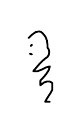
\begin{tikzpicture}[x=.3mm,y=.3mm,line cap=round,line join=round]\draw[line width=.65pt] (0,25) .. controls (2,27) and (4,29) .. (6,27) .. controls (8,25) and (8,23) .. (8,21) .. controls (9,20) and (9,18) .. (8,17) .. controls (5,15) and (3,12) .. (2,11) .. controls (4,10) and (7,13) .. (9,13) .. controls (9,11) and (6,8) .. (5,7) -- (5,5) .. controls (7,7) and (9,7) .. (10,6) -- (10,3) .. controls (9,1) and (8,0) .. (7,-2) -- (9,-2);\draw[line width=.7pt] (1.4,22.1) -- (1,21.7);\draw[line width=.7pt] (.6,18.3) -- (1.4,18.1);\end{tikzpicture}}}sur $\handwritten{\Lambda}$.( \inserted{\handwritten{qui est \unsure{cohérent|abélienne|abélien} bien que $\Lambda$ ne soit pas \unsure{noethérien|noéthérien}, car $\Lambda$ est}} \deleted{est-il noethérien, j.e. le nombre de générateurs est-il
fini ? )}\handwritten{ $\underset{\unsure{\rightharpoondown|\longrightarrow}}{\lim}$ d'anneaux noeth\unsure{.|,} à hom de transition \uline{plats} )}.

Cette construction ressemblerait à celle d'une théorie des
motifs où on n'aurait pas passé à l'équivalence homologique pour
les cycles, mais où on aurait gardé l'équivalence rationelle, - qui
est bien trop fine \deleted{p\unsure{ou|eu}}à beaucoup d'égards. Pour trouver un équiva
lent plus étroit, il convin\unsure{\deleted{t}n|\deleted{n}t}t de reprendre la théorie prédédente,on
pourrait formuler le même Pb universel que plus haut, mais en prena
l'équivalence homologique (via le graphe) des morphismes de variété
au lieu de l'équivalence homotopique. \deleted{Mais alors il semble que l'on
trouve comme catégorie solution celle dont les objets sont les vari}

\margin{\handwritten{15}}
